
% This LaTeX was auto-generated from MATLAB code.
% To make changes, update the MATLAB code and republish this document.

\documentclass{article}
\usepackage{graphicx}
\usepackage{color}

\sloppy
\definecolor{lightgray}{gray}{0.5}
\setlength{\parindent}{0pt}

\begin{document}

    
    
\subsection*{Contents}

\begin{itemize}
\setlength{\itemsep}{-1ex}
   \item Preambles
   \item Load the data
   \item Initialise Km and meanKm
   \item We get a community matrix for 10,20, and 30 clusters
   \item Boxplot of data
\end{itemize}


\subsection*{Preambles}

\begin{verbatim}
clear all; close all; clc;
savePlots = 1;
\end{verbatim}


\subsection*{Load the data}

\begin{verbatim}
load('cbt3data.mat');
\end{verbatim}


\subsection*{Initialise Km and meanKm}

\begin{verbatim}
person_type = {'Diseased Patients';'Healthy Controls'};
D_diseased_total = [];
D_healthy_total = [];
\end{verbatim}


\subsection*{We get a community matrix for 10,20, and 30 clusters}

\begin{verbatim}
for K = 1:3:70;
    tic;
    % we get the ith diseased and healthy person
    X = diseased(:,:,1)';
    Y = healthy(:,:,1)'; % we get the ith healthy person

    % For the ith person, we get the cluster index for each brain region
    [~,~,~,D_diseased] = kmeans(X,K, 'Replicates',100);
    [~,~,~,D_healthy] = kmeans(Y,K, 'Replicates',100);

    % We take the distance closest to a cluster
    D_diseased_min = min(D_diseased,[],2);
    D_healthy_min = min(D_healthy,[],2);

    % We store the ditances for each point to its respective mean
    D_diseased_total = [D_diseased_total, D_diseased_min];
    D_healthy_total = [D_healthy_total, D_healthy_min];

end
\end{verbatim}


\subsection*{Boxplot of data}

\begin{verbatim}
figure(1)
boxplot(D_diseased_total);
labels = (1:3:60);
set(gca, 'XTickLabel', labels);
% set(gca,'YScale','log')
xlabel('Number of cluster, K','fontsize',16);
ylabel('Log distance to closest mean','fontsize',16);
title('Elbow plot for optimum K of diseased patients', 'fontsize',18);
if (savePlots == 1)
    filename = ('elbowDiseased.png');
    saveas(gcf,filename);
end

figure(2)
boxplot(D_healthy_total);
labels = (1:3:90);
set(gca, 'XTickLabel', labels);
set(gca, 'XTickLabel', labels);
% set(gca,'YScale','log')
xlabel('Number of cluster, K','fontsize',16);
ylabel('Log distance to closest mean','fontsize',16);
title('Elbow plot for optimum K of healthy controls', 'fontsize',18);
if (savePlots == 1)
    filename = ('elbowHealthy.png');
    saveas(gcf,filename);
end
\end{verbatim}

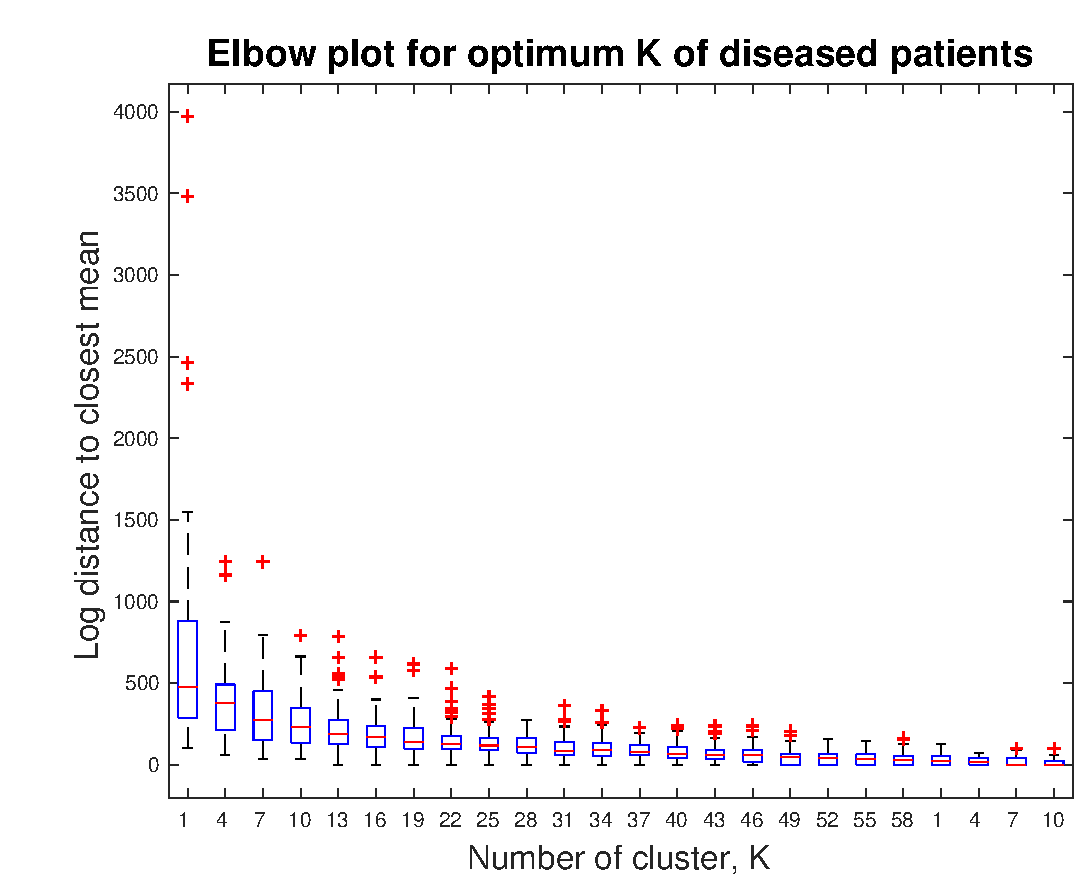
\includegraphics [width=4in]{cbt3_cluster_experimentation_01.eps}

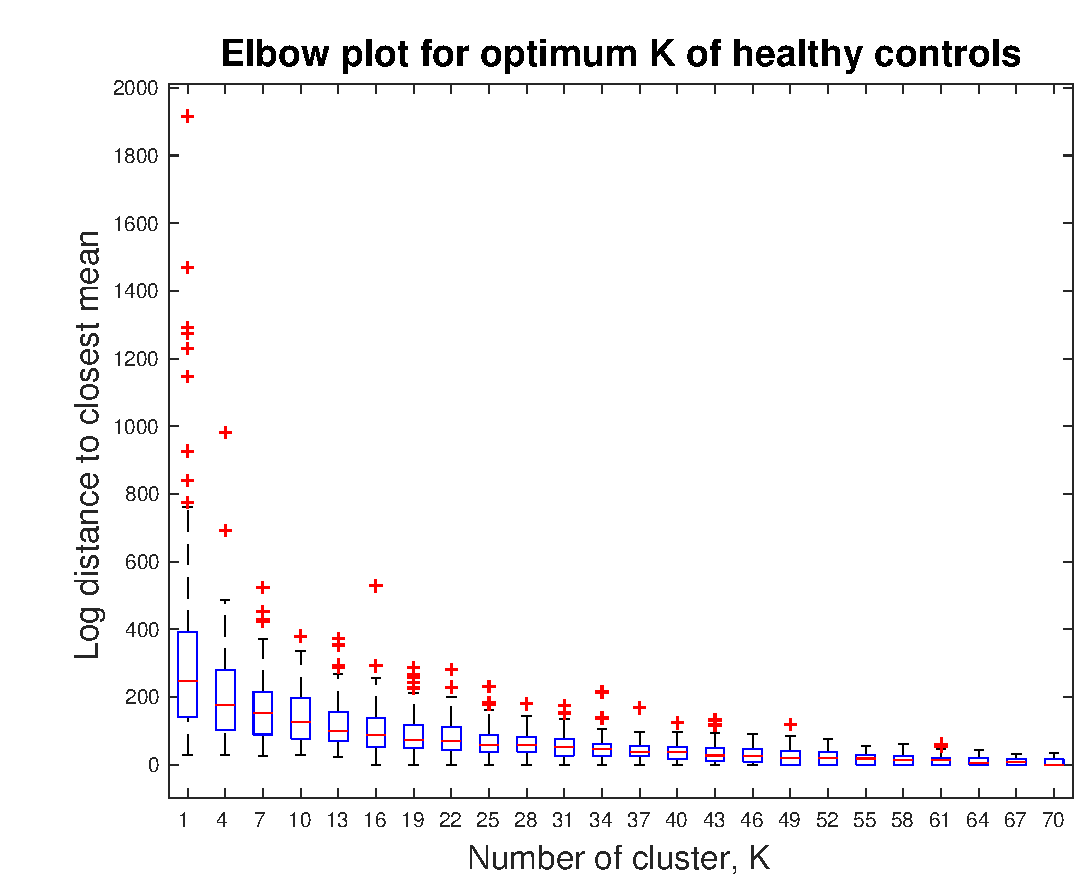
\includegraphics [width=4in]{cbt3_cluster_experimentation_02.eps}



\end{document}
    
